\documentclass[a4, 12pt, addpoints]{exam}
\usepackage[margin=0.9in, top = 2cm]{geometry}
\usepackage[utf8]{inputenc}
\usepackage{graphics}
\usepackage{color}
\usepackage{amssymb}
\usepackage{amsmath}
\usepackage{enumitem}
\usepackage{xcolor}
\usepackage{cancel}
\usepackage{ragged2e}
\usepackage{graphicx}
\usepackage{multicol}
\usepackage{color}
\usepackage{tikz}
\usepackage{circuitikz}
\usepackage{siunitx}
\usepackage{longtable}
\usepackage{float}
\usepackage{parskip}
\usepackage{caption, subcaption}
\CorrectChoiceEmphasis{\itseries\color{red}}

\runningfooter%
    {}
    {\textbf{D.I.E.T., Satara}}
    { \thepage
    %\iflastpage{}{
%        \textbf{Question \thequestion }%
%        \ifcontinuation{ -- continued}{}\\%
%        \oddeven{\textbf{TURN OVER}}{}
%        }
    }
%MOVE THIS FOOTER TO THE RIGHT BY 0.4in, same for the header, but I've left it out as the header is even longer which lots of if conditions.

\pagestyle{headandfoot}
\begin{document}
\def\arraystretch{1}
\begin{longtable}{lp{0.65\textwidth}p{0.15\textwidth}r}
\multicolumn{4}{c}{
\includegraphics[width= \textwidth]{dietlogo}} \\ 
\multicolumn{4}{c}{Written Test for Degree Engineering Interview} \\
Date:20/07/2024 & \multicolumn{2}{c}{ ~~~Branch: E \& TC Engineering ~~~~ Time:1 hr} & Marks:20 \\
\multicolumn{4}{l}{ Note: All questions are compulsory and carry 2 marks each  } \\ \hline
\end{longtable}
%\vspace{0.1in}
\begin{questions}
%\section*{\normalsize Q.1 to Q.20 carry 1 mark each}
%\question If silicon diode is operating in forward bias in a circuit with 12 V supply and 240 $\Omega$ series resistance, then what is the voltage drop across the diode. \\[0.3cm]
%\begin{oneparchoices}
%\choice 1.5 V
%\choice 0.4 V
%\choice 1.1 V
%\choice 0.7 V
%\end{oneparchoices}  
%\question Which of the following is the trivalent doping element?:\\[0.3cm]
%\begin{oneparchoices}
%\choice Arsenic
%\choice Boron
%\choice Phosphorous
%\choice Antimony
%\end{oneparchoices}  
%\question The ripple factor for the bridge rectifier is:\\[0.3cm]
%\begin{oneparchoices}
%\choice 0.406
%\choice 1.21
%\choice 1.10
%\choice 2.22
%\end{oneparchoices}  
%\question According to barkhausen criteria the loop gain $\beta v$ of the oscillator must be equal to --------.\\[0.3cm]
%\begin{oneparchoices}
%\choice 0
%\choice 1
%\choice 0.8
%\choice -1
%\end{oneparchoices}
%\question When PN junction is forward biased:\\[0.3cm]
% \begin{oneparchoices}
%\choice Deletion region decreases
%\choice Minority carriers are not affected
%\choice Holes and electrons moves away from each other
%\choice All of above.
%\end{oneparchoices} 
%\question According to boolean algebraic theorem  the expression $A (A + B)$ is equivalent to: \\[0.3cm]
% \begin{oneparchoices}
%\choice $\pmb{A + B} $ 
%\choice $\pmb{B}$
%\choice $\pmb{A}$
%\choice $\pmb{AB}$
%\end{oneparchoices} 
%\question The decimal number representation of the following number $ (1~1~0~1~0~1)_2 $ is: \\[0.3cm]
%\begin{oneparchoices}
%\choice $ (53)_{10} $ 
%\choice $ (12)_{10} $
%\choice $ (45)_{10}$
%\choice $ (67)_{10} $
%\end{oneparchoices} 
%\question Which among the following is a current controlled device?\\[0.3cm]
%\begin{oneparchoices}
%\choice MOSFET
%\choice BJT
%\choice IGBT
%\choice JFET
%\end{oneparchoices} 
%\question The storage delay time can be reduced considerably by preventing transistor from going into saturation. This is achieved by connecting the schottky diode between -------- and --------:\\[0.3cm]
%\begin{oneparchoices}
%\choice Base and Collector
%\choice Base and Emitter
%\choice Emitter and Collector
%\choice In series with Base. 
%\end{oneparchoices}  
%\question Gate to Source voltage must be ------- the threshold voltage for enhancement type MOSFET to be cut off.\\[0.3cm]
%\begin{oneparchoices}
%\choice Greater than
%\choice Equal to
%\choice Less than
%\choice All of the above
%\end{oneparchoices}  
%\question An equivalent base 2 number of $(13)_{10}$ is:\\[0.3cm]
%\begin{oneparchoices}
%\choice $(0~1~0~1)_2$ 
%\choice $(1~1~0~1)_2$
%\choice $(1~1~1~1)_2$
%\choice $(1~0~0~1)_2$
%\end{oneparchoices} 
%\question The voltage across $660 \Omega$ resistance is (refer Figure~\ref{fig:2}):
%\begin{figure}[H]
%\centering
%\resizebox{0.38\textwidth}{!}{
%\begin{circuitikz}[american ]
%\draw
%(0,0) to [short, i=$I_x$] (0,4)
%      to [R, l= $330 \Omega$] (4,4)
%      to [R, l= $660 \Omega$] (8,4)
%      to [short]  (8,0);
%\draw      
%(0,0) to [V, v= $3V$] (8,0);
%\draw
%(4,4) to [short] (4,3)
%      to [R, l_= $660 \Omega$] (8,3);
%
%\end{circuitikz}}
%\caption{Q.12}
%\label{fig:2}
%\end{figure}
%\begin{oneparchoices}
%    \choice $0.65 V$
%    \choice $1.5 V$
%    \choice $0.72 V$
%    \CorrectChoice $0.75 V$
%    
%\end{oneparchoices}
%\question The current $I_x$ and $I_y$ are (refer Figure~\ref{fig:3}).
%\begin{figure}[H]
%\centering
%\resizebox{0.38\textwidth}{!}{
%\begin{circuitikz}[american]
%\draw
%(0,0) to [isource, l=$1A$] (4,0)
%      to [R, l= $5 \Omega$, i=$I_x$] (8,0)
%      to [short] (8,2)
%      to [short] (4,2)
%      to [isource, l=$5A$] (4,0)
%      to [R, l = $1 \Omega$, i=$I_y$] (4, -3)
%      to [short] (0, -3)
%      to [short] (0,0);
%\end{circuitikz}}
%\caption{Q.13}
%\label{fig:3}
%\end{figure}
%\begin{oneparchoices}
%    \choice $-1A, 5A$
%    \choice $ 5A, 1A$
%    \choice $1A, 5A$
%    \CorrectChoice $5A, -1A$
%\end{oneparchoices}    
%\question  Which of the following is not a property of semiconductors used in electronic devices?\\[0.3cm]
%\begin{oneparchoices}
%\choice They excite electrons
%\choice They don't emit light
%\choice They have high thermal conductivity
%\choice They have variable electrical conductivity  
%\end{oneparchoices}  
%\question Which of the following is the correct relationship between temperature $(T)$ and mobility $(\mu)$ of electrons in electronic circuits?\\[0.3cm]
%\begin{oneparchoices}
%\choice $\mu \propto T^{-3/2} $
%\choice $ \mu \propto T^{-1/2} $
%\choice $ \mu \propto T $
%\choice $ \mu \propto T^{-1} $  
%\end{oneparchoices}  
%\question What type of semiconductor is used in LED electronic circuits?\\[0.3cm]
%\begin{oneparchoices}
%\choice Intrinsic semiconductor
%\choice Compound semiconductor
%\choice Degenerated semiconductor
%\choice Compensated semiconductor
%\end{oneparchoices}
%\question  The equivalent resistance of the circuit given in Figure~\ref{fig:6} is given by
%\begin{figure}[H]
%\centering
%\resizebox{0.38\textwidth}{!}{
%\begin{circuitikz}[american, scale=0.8]
%\draw
%(-1,0) to [short, o-] (0,0);
%\draw
%(0,0) to [R, l=$1\textrm{k}\Omega$] (2,0)
%      to [R, l=$1\textrm{k}\Omega$] (6,0)
%      to [R, l=$3\textrm{k}\Omega$] (10,0)
%      to [R, l=$5\textrm{k}\Omega$] (14,0)
%      to [short] (15,0)
%      to [short] (15,-4)
%      to [short, -o] (-1,-4);
%\draw
%(3,-1) to [R, l_=$1\textrm{k}\Omega$] (5, -1);
%\draw
%(3, -1) to [short] (3,0);
%\draw
%(5, -1) to [short] (5,0);
%\draw
%(7,-1) to [R, l_=$3\textrm{k}\Omega$] (9, -1);
%\draw
%(7, -1) to [short] (7,0);
%\draw
%(9, -1) to [short] (9,0);
%\draw
%(11,-1) to [R, l_=$5\textrm{k}\Omega$] (13, -1);
%\draw
%(11, -1) to [short] (11,0);
%\draw
%(13, -1) to [short] (13,0);
%\end{circuitikz}}
%\caption{Q.17}
%\label{fig:6}
%\end{figure}
%\begin{oneparchoices}
%    \choice $\SI{4}{k\Omega}$
%    \CorrectChoice $\SI{10}{k\Omega}$
%    \choice $\SI{5.5}{k\Omega}$
%    \choice $\SI{5}{k\Omega}$
%\end{oneparchoices}
%\question In the circuit shown in Figure~\ref{vc} below, $V_1$ and $V_2$ are bias voltages. Based on input and output impedances, the circuit behaves as a
%\begin{figure}[h!]
%\centering
% \begin{circuitikz}[american,]
%\ctikzset{tripoles/mos style=arrows}
%\ctikzset{transistors/arrow pos=end}
% \ctikzset{tripoles/pmos style/nocircle}
% \draw (0,0)  node[pmos](Q1){Q1}
% 
%(Q1.source) to [short] (0,1)
%--(0,1)  node[vcc](VDD){$V_{DD}$};
%
%\draw 
%++(0,-2)  node[nmos](Q2){Q2}   ;
%\draw
%(Q1.drain) to [short] (Q2.drain);
%\draw
%(Q2.source) to [short] (0,-3)
%            to [R, l=$R_l$] (0,-5)
%            to [sV, l=$V_{IN}$]  (0,-7)  
% (0,-7) node[ground](GND){}; 
% \draw
% ++(Q2.drain)  to [short, -o, l=$V_{OUT}$] (1,-1.23);               
% \draw
%(Q1.gate) to [short, -o, l=$V_1$](-1,0);
%\draw
%(Q2.gate) to [short, -o, l=$V_2$](-1,-2);
%\end{circuitikz}
%\caption{Q.18}
%\label{vc}
%\end{figure}
%~\\[0.3cm]
%\begin{oneparchoices}
%\choice voltage controlled voltage source.
%\choice voltage controlled current source.
%\choice current controlled voltage source.
%\choice current controlled current source.
%\end{oneparchoices}
%\question If silicon diode is operating in forward bias in a circuit with 12 V supply and 240 $\Omega$ series resistance, then what is the voltage drop across the diode. \\[0.3cm]
%\begin{oneparchoices}
%\choice 1.5 V
%\choice 0.4 V
%\choice 1.1 V
%\choice 0.7 V
%\end{oneparchoices}  
%\question A digital communication system transmits a block of $N$ bits. A probability of error in decoding a bit is $\alpha$. The error event of each bit is independent of error event of other bits. Received block is declared erroneous if atleast on of its bits decoded wrongly. The probability that the received block is erroneous is:\\[0.3cm]
%\begin{oneparchoices}
%\choice $N(1-\alpha)$
%\choice $\alpha^N$
%\choice $1 - \alpha^N $
%\choice $ 1- (1 - \alpha)^N$
%\end{oneparchoices}     
%=========================================================
%\section*{\normalsize Q.21 to Q.30 carry 2 marks each}
\question Let $m(t)$ be a strictly band-limited signal with bandwidth $B$ and energy $E$. Assuming $\omega_0 = 10B$, the energy in the signal $m(t) \cos \omega_0 t$ is\\[0.3cm]
\begin{oneparchoices}
\choice $\dfrac{E}{4}$
\choice $\dfrac{E}{2}$
\choice $E$
\choice $2E$
\end{oneparchoices}  
\question In feedback control system shown in Figure~\ref{q2} below $ G(s) = \dfrac{6}{s(s+1)(s+2)} $, where $R(s), Y(s), \& E(s)$ are Laplace transform of $r(t), y(t), \& e(t) $ respectively, if the input $r(t)$ is a unit ramp function then ------  \\[0.3cm]
\begin{oneparchoices}
\choice $\lim \limits_{t \to \infty } e(t) = 0$
\choice $\lim \limits_{t \to \infty } e(t) = \dfrac{1}{3}$
\choice $\lim \limits_{t \to \infty } e(t) = \dfrac{1}{4}$
\choice $\lim \limits_{t \to \infty } e(t) $ does not exist, $e(t)$ is oscillatory.
\end{oneparchoices}
\begin{figure}[h!]
\centering
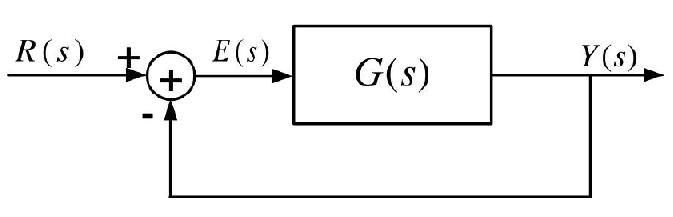
\includegraphics[width=0.5\textwidth]{fbc.png}
\caption{Q.22}
\label{q2}
\end{figure}  
\question What is the z-transform of the following finite duration signal? $ x[n] = \{ 2, 4, \underset{\uparrow}{5}, 7, 0, 1 \} $\\[0.3cm]
\begin{oneparchoices}
\choice $ 2 + 4z + 5z^2 + 7z^3 + z^4  $
\choice $2 + 4z + 5z^2 + 7z^3 + z^5$
\choice $ 2 + 4z^{-1} + 5z^{-2} + 7z^{-3} + z^{-5} $
\choice $ 2z^2 + 4z + 5 +7z^{-1} + z^{-3}$
\end{oneparchoices}  
\question The BJT as a switch is  operated in one of the following:
\begin{oneparchoices}
\choice Only saturation region
\choice Active region
\choice Only cut off region
\choice Both saturation and cut off region
\end{oneparchoices}  
\question A DC power supply has no load voltage of 30 V and full load voltage of 25 V at full load current of 1 A. Its output resistance and load regulation respectively are. \\[0.3cm]
\begin{oneparchoices}
\choice $5 \Omega$ and $20 \%$ 
\choice $25 \Omega$ and $20 \%$
\choice $5 \Omega$ and $ 16.7 \%$
\choice $25 \Omega$ and $16.7 \%$
\end{oneparchoices} 
\question A 500 W carrier signal is amplitude modulated with modulation percentage of 60\%.  The total power in the modulated signal if the amplitude modulation used is  the double sideband AM with full carrier(A3E) is. \\[0.3cm]
 \begin{oneparchoices}
\choice 590 W
\choice 534 W
\choice 125 W
\choice 300 W
\end{oneparchoices} 
\question What will be the o/p of the given logic gate of Figure~\ref{lg}?
\begin{figure}[H]
\centering
\resizebox{0.36\textwidth}{!}{
\begin{circuitikz}[american voltages]
\draw
 
 (0,2) node[nor port] (mynor1) {}
(0,0) node[nor port] (mynor2) {}
(2,1) node[nor port] (mynor) {}
(mynor1.out) -- (mynor.in 1)
(mynor2.out) -- (mynor.in 2)
(4,1) node[nor port] (mynor3) {}
(mynor3.west) -- (mynor.out)
(mynor3.in 1) -- (mynor3.in 2)
(mynor1.in 1) -- (mynor1.in 2)
(mynor2.in 1) -- (mynor2.in 2)
(mynor1.west) -- (-2,2)
(mynor2.west) -- (-2,0)
(-2.2,2) node{A}
(-2.2,0) node{B}
(mynor3.east) node {~~~Q} ;  
\end{circuitikz}}
\caption{Q.27}
\label{lg}
\end{figure}
\begin{oneparchoices}
\choice NOR
\choice NAND
\choice AND
\choice OR
\end{oneparchoices} 
\question Let $\hat{i}$ and $\hat{j}$ be the unit vectors along $x$ and $y$ axes respectively, and let $A$ be the positive constant. Which one of the following is true for vector fields $ \bar{F_1} = A ( \hat{i} y + \hat{j} x ) $, $ \bar{F_2} = A ( \hat{i} y - \hat{j} x ) $  \\[0.3cm]
\begin{oneparchoices}
\choice Both $\bar{F_1}$ and $\bar{F_2}$ are electrostatic fields.
\choice Only $\bar{F_1}$ is an electrostatic fields.
\choice Only $\bar{F_2}$ is an electrostatic fields.
\choice Neither $\bar{F_1}$ nor $\bar{F_2}$ are electrostatic fields.
\end{oneparchoices} 
\question The current $I_y$ flowing through $660 \Omega$ resistance  is (Refer Figure~\ref{fig:1}):
\begin{figure}[H]
\centering
\resizebox{0.33\textwidth}{!}{
\begin{circuitikz}[american voltages]
\draw
(0,4) to [V, v_= $3V$, i = $I_x$] (0,0);
\draw
 (0,4)     to [short]      (3,4)
      to [R, i= $I_y$, l=$660 \Omega$] (6,4);
\draw
(0,0) to [R, l=$330\Omega$] (3,0);
\draw
(3,4) to [short] (3,3)
      to [R, l=$660\Omega$] (6,3)
      to [short] (6,4);
\draw
(6,3) to [short] (3,0)
      to [R, l_=$330 \Omega$] (0,4);      
\end{circuitikz}}
\caption{Q.29}
\label{fig:1}
\end{figure}

\begin{oneparchoices}
    \choice $I_x$
    \choice $I_x/2$
    \CorrectChoice $I_x/4$
    \choice $I_x/3$
\end{oneparchoices}

\question In the circuit shown below, P and Q are the inputs. The logical function realized by the circuit shown Figure~\ref{fig:2} below is:
\begin{figure}[H]
\centering
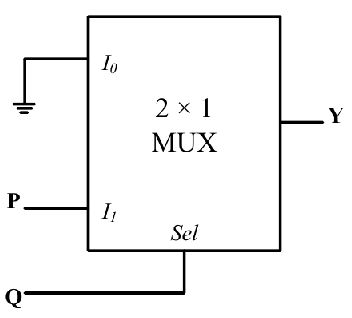
\includegraphics[width=0.23\textwidth]{mux}
\caption{Q.30}
\label{fig:2}
\end{figure}
\begin{oneparchoices}
    \choice $Y = PQ$
    \choice $Y=P+Q$
    \choice $Y = \overline{PQ}$
    \CorrectChoice $Y= \overline{P + Q}$
    
\end{oneparchoices}



\vspace{0.10in}

\end{questions}
\end{document}
 